
%%%%%%%%%%%%%%%%%%%%%%%%%%%%%%%%%%%%%%%%%%%%%%%%%%%%%%%%%%%%%%%%%%%%
\section{DAQ Design}
\label{sec:fdsp-daq-design}

\metainfo{16 Pages}


%%%%%%%%%%%%%%%%%%%%%%%%%%%%%%%%%%%
\subsection{Overview (Giles Barr)}
\label{sec:fdsp-daq-ltr}

Here we describe the overall readout and data acquistion
strategy. This will include the high-level data flow diagram,
(Figure~\ref{fig:daq-readout-buffering-baseline} may be sufficient)
which is divided in functional boxes, each of which are described in
turn in the sections below.

%%%%%%%%%%%%%%%%%%%%%%%%%%%%%%%%%%%
\subsection{Local Readout \& Buffering (Giles Barr \& Brett Viren)}
\label{sec:fdsp-daq-ltr}

\metainfo{Describe how the data is received from the detector electronics, and buffered while awaiting a trigger decision, together with any processing that affects stored data.  The starting point is data incoming from the WIBs and the end point is corresponding data sitting in memory ready for event building. }

Figure~\ref{fig:daq-readout-buffering-baseline} illustrates the local
readout and buffering data flow in the context of a single APA.  

\begin{dunefigure}[Baseline Readout and Buffering]{fig:daq-readout-buffering-baseline}
  {Illustration of data flow from Cold Electronics WIBs through RCE,
    FELIX, RAM buffer for one APA.  The buffer in each APA DAQ Front
    End system will then be polled by the Single-Phase Event Builder
    process which services all 150 APAs.  \fixme{Note, this assumes trigger primitives are sent along with data which still a point of discussion.  When decided, this diagram may need changes.}}
% This PDF is made from the .dot of the same name.
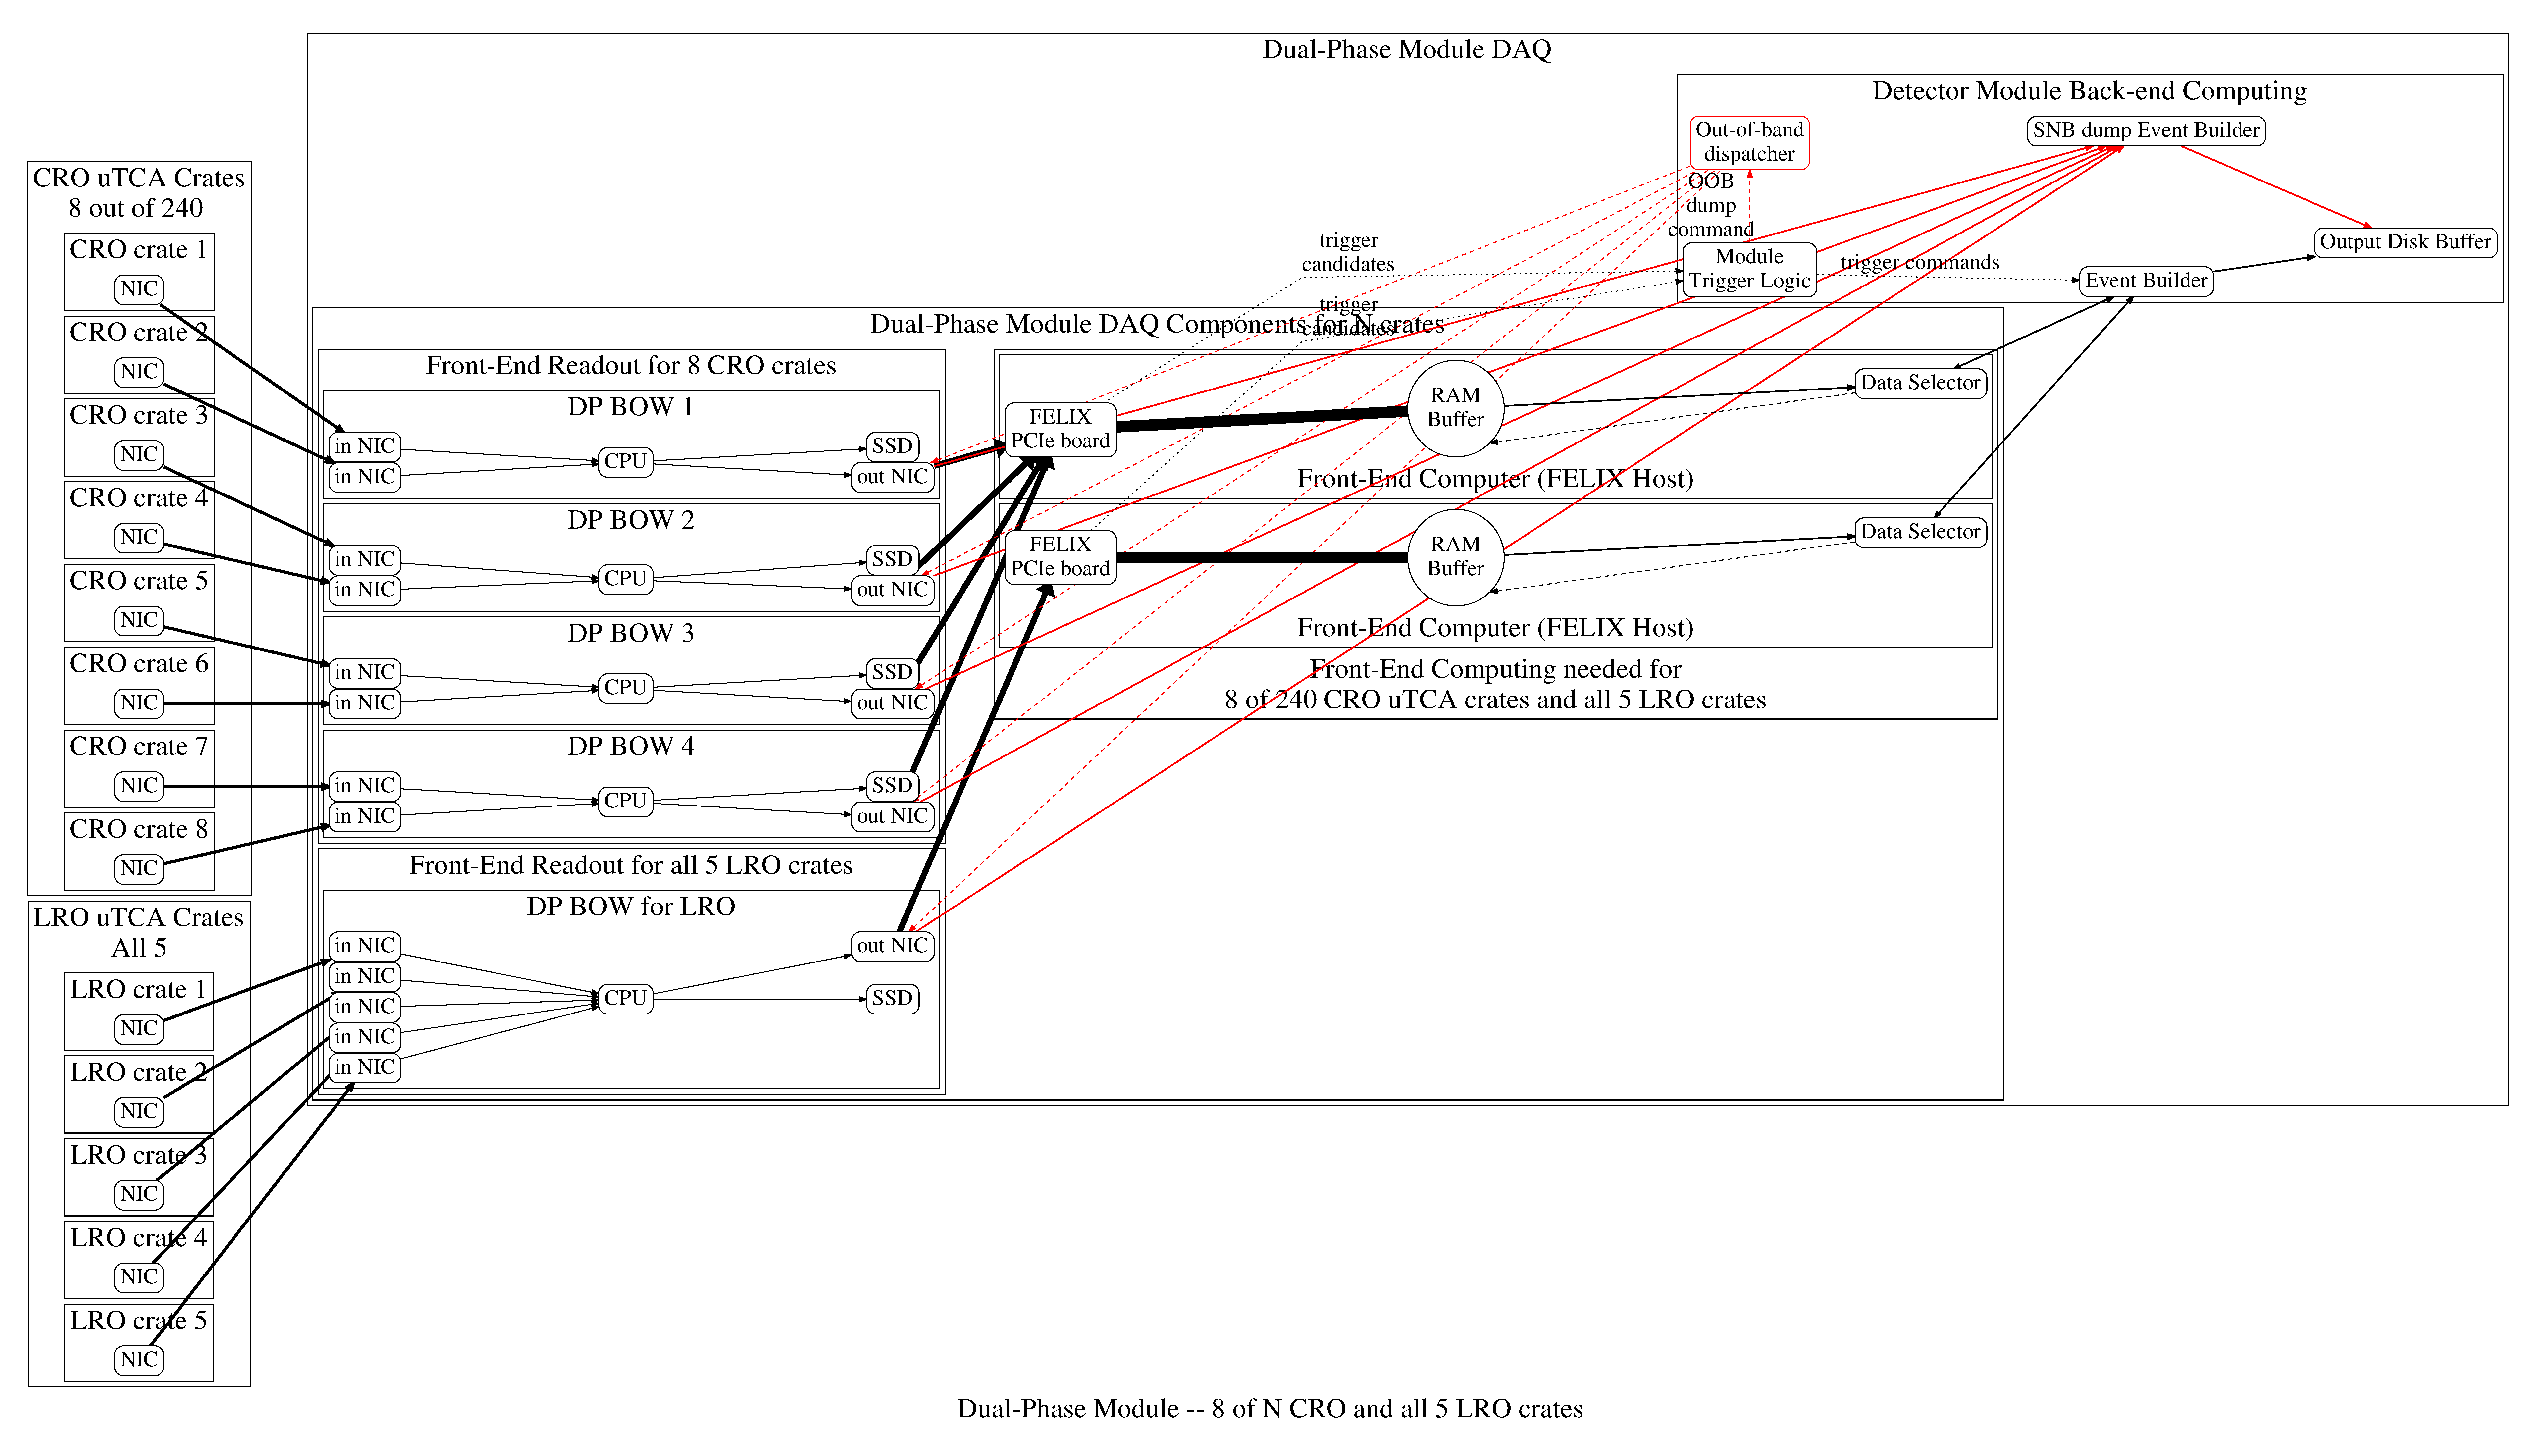
\includegraphics[width=0.8\textwidth]{daq-readout-buffering-baseline.pdf}%
\end{dunefigure}


%%%%%%%%%%%%%%%%%%%%%%%%%%%%%%%%%%%
\subsection{Local Trigger Primitive Generation (Josh Klein \& Brett Viren)}
\label{sec:fdsp-daq-ltr}

\fixme{Below are from slides bv may show at the Jan WS.  Content copied here and now as a starting point.}

The TPC data is used to generate \textit{trigger primitive messages}
(TPM) local to each APA and which summarize the activity recently
sensed by their connected conductors.  These TPMs are emited from each
APA DAQ Front End and become fodder for later determining
\textit{trigger command messages} (TCM) as described in
Section~\ref{sec:fdsp-daq-sel}.

Only the 480 collection channels associated with each APA face are
used for forming TCMs.  Reasons for this reduction include the fact
that collection channels:

\begin{itemize}
\item have higher signal to noise ratio compared to induction channels.
\item fully and independently are sensitive to each APA face.
\item have unipolar signals that directly give an approximate measure
  of ionization charge without costly field response deconvolution
  computation.
\item can be divided into smaller groups defined by natural hardware
  boundaries for parallel processing.
  % fixme: do we need a statement about efficiency here?
\end{itemize}


Figure~\ref{fig:daq-overview} illustrates the connectivity between the
four connectors on each of the five WIBs and the DAQ APA Front End.
The data is received from 80 1 Gbps fiber optical links by four
Reconfigurable Computing Elements (RCE) in the ACTA Cluster On Board
(COB) system. \fixme{Matt: help!  Each RCE consists of a ....}

The pattern of connectivity between WIBs and RCEs results in the data
from the collection channels covering one half of one APA face being
received by each RCE.  Each RCE has two primary functions.  The first
is transmission of all data as described in
Section~\ref{sec:fdsp-daq-hlt}.  The second is to produce TPMs from
its portion of the collection channel data.

The TPMs are produced from a \textit{trigger primitive production
  pipeline} of algorithms.  These algorithms still require development
but can be broadly described.   

\begin{enumerate}
\item On a per channel basis calculate a rolling baseline and RMS that
  characterizes recent samples minimal influence from ionization
  signal.
\item Locate contiguous ADC samples that go above a threshold which is
  defined in terms of the baseline and RMS.
\item Emit their time bounds and total charge as a $ROI_{ch}$ TPM.
\end{enumerate}

These $ROI_{ch}$ TPM represent some possible activity occurring
somewhere in the LAr within a $\pm$\SI{2.5}{\mm} strip that extends in
time by the ROI time bounds.  Depending on the threshold set, these
TPMs may be numerous due to \Ar39 decays and noise fluctuations.
Further processing must be done with more global information.  This
may be done as part of the Module Trigger Logic (MTL) as described in
Section~\ref{sec:fdsp-daq-sel} or it may be done immediately in the
RCE pipeline.  Strategies to summarize these detailed TPM into fewer
TPMs include:

\begin{enumerate}
\item Pad each $ROI_{ch}$ in a channel by a fixed amount in order to
  anticipate their use later as defining readout (eg, long enough to
  account for inter-plane drift times (\SI{6.25}{\micro\second}) and
  induction signal extents ($\sim$\SI{100}{\micro\second}).
\item Form the union of ROI across all channels observed by a given RCE.
\item Merge subsequent ROI which are separated by some small time
  interval.
\end{enumerate}

If the Single-Phase detector module generates excess noise, such as
that from RF emission picked up coherently across some group of
channel, it must be mitigated at the start of the pipeline and will
likely require additional computational resources.  Some ideas to
respond to this scenario include....\fixme{Ideas?}.



%%%%%%%%%%%%%%%%%%%%%%%%%%%%%%%%%%%
\subsection{Dataflow (Giles Barr \& Josh Klein \& Brett Viren)}
\label{sec:fdsp-daq-hlt}

\metainfo{Describe the dataflow {\it infrastructure}. This should cover buffer and transport of data and trigger information, infrastructure for generating local and global trigger commands (but not their algorithms, that's next), as well as what happens to the data once a trigger is generated (ie. event building).
Figure~\ref{fig:daq-readout-buffering-baseline} may be referenced}


%%%%%%%%%%%%%%%%%%%%%%%%%%%%%%%%%%%
\subsection{Data Selection Algorithms (Josh Klein \& Brett Viren)}
\label{sec:fdsp-daq-sel}

This section describes the strategy for using the trigger/dataflow infrastructure, with example algorithms.

\metainfo{Describe Module Trigger Logic and Global Trigger Logic.
  Describe creation of Trigger Command Messages (TCM) from TPMs.
  Included external sources of TPMs such as SNEWS, Fermilab Beam,
  testing triggers, periodic triggers, calibration triggers.}

\metainfo{Here should go the assumptions that went into the thinking
  for Josh's event category data volumes.  It can include discussion
  of tighter selection criteria for ``cosmics'' such as Phil's
  distribution of number of APAs hit by cosmics and arguments for
  something less than 2+ drift time readouts.}

%
% %%%%%%%%%%%%%%%%%%%%%%%%%%%%%%%%%%%
% \subsection{High-Level Trigger}
% \label{sec:fdsp-daq-eb}
%
% Data selection after event building.
%

\subsection{Timing \& Synchronization}
\label{sec:fdsp-daq-hlt}

Describe the generation of timing/synchronisation signals and and distribution to the detectors.


%%%%%%%%%%%%%%%%%%%%%%%%%%%%%%%%%%%
\subsection{Computing \& Network Infrastructure}
\label{sec:fdsp-daq-infra}

Describes the infrastructure that will support the software components described above.

%%%%%%%%%%%%%%%%%%%%%%%%%%%%%%%%%%%
\subsection{Run Control \& Monitoring}
\label{sec:fdsp-daq-tcm}

Describe how the system is controlled and monitored.

